\section{绪论}

\subsection{最优化简介}
优化问题可以表示成
\[
    \begin{array}{c}
        \min f(\boldsymbol{x})\\
        \operatorname{s.t.} \boldsymbol{x}\in \Omega
    \end{array}
\]
可行域有多种表达形式,一般用等式和不等式定义,即
\[
    \Omega = \left\{ \boldsymbol{x}\in\mathbb{R}^n|c_{i}(\boldsymbol{x}) = 0,i\in \mathcal{E};\ c_{i}(\boldsymbol{x})\geqslant 0,i\in\mathcal{I}  \right\}
\]

\begin{note}
    线性问题:
    \begin{figure}[htbp]
        \centering
        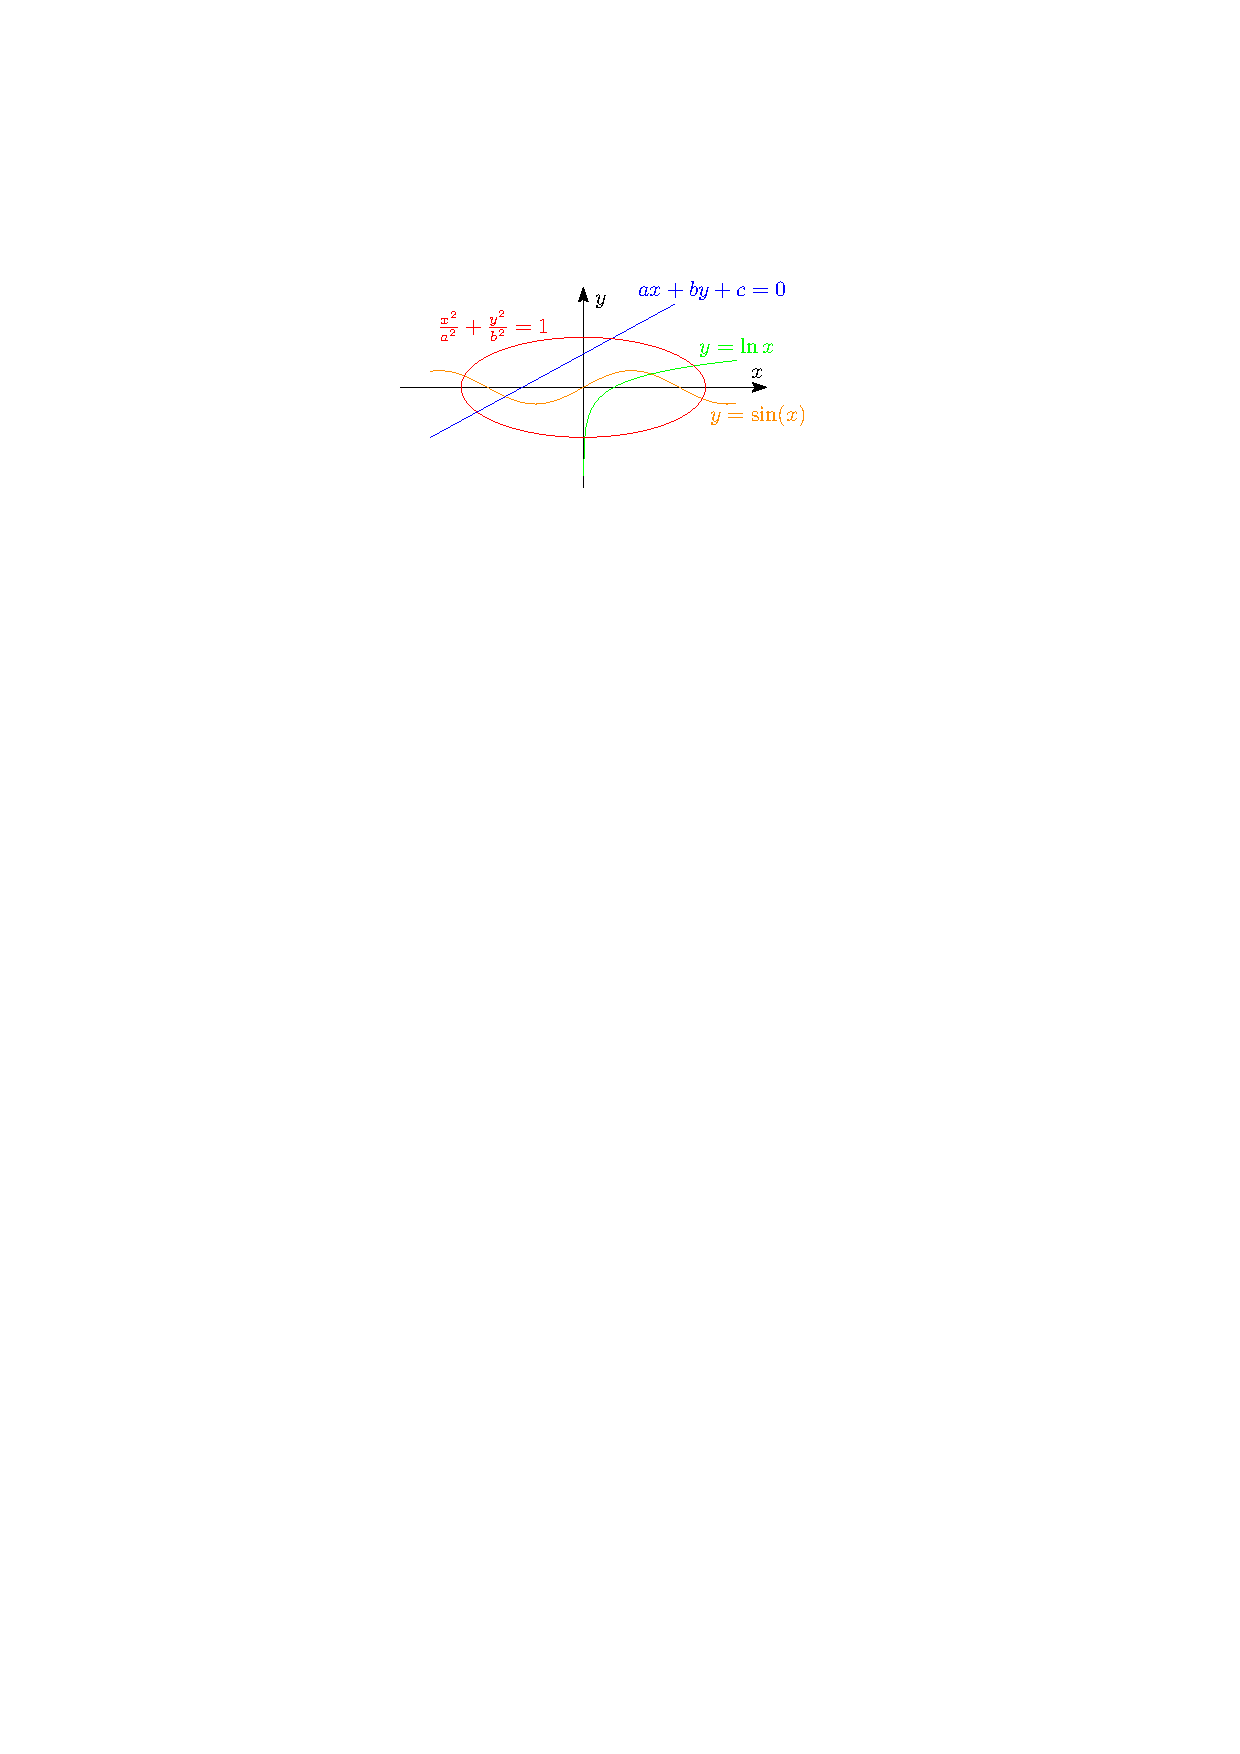
\includegraphics{image/线性.pdf}
    \end{figure}
    \begin{itemize}
        \item 线性规划
        \[
            \begin{array}{c}
                \min\ \boldsymbol{c}^{\mathrm{T}}\boldsymbol{x}\\
                \operatorname{s.t.} \boldsymbol{Ax} = 0\\
                \boldsymbol{x}\geqslant 0
            \end{array}
        \]
        \item 非线性规划
        \[
            \begin{array}{c}
                \min\ \dfrac{1}{2}\boldsymbol{x}^{\mathrm{T}}\boldsymbol{Gx}+\boldsymbol{g}^{\mathrm{T}}\boldsymbol{x}\\
                \operatorname{s.t.} \boldsymbol{A}_1\boldsymbol{x} = \boldsymbol{b}_1\\
                \boldsymbol{A}_2\boldsymbol{x} \geqslant \boldsymbol{b}_2
            \end{array}
        \]
    \end{itemize}
\end{note}
\begin{example}
    若目标函数在可行域上有下界,但无最优解,则目标函数在可行域上的下确界成为优化问题的最优值。
    \[
        \operatorname{inf}\left\{ f(\boldsymbol{x})| \boldsymbol{x}\in \Omega \right\}
    \]

    如二元函数$f(\boldsymbol{x}) = x_1^2+(1-x_1x_2)^2$在$\mathbb{R}^2$上的最优值为0,但只有在$x_1 = \frac{1}{x_2}$且$x_2\to \infty$是才能达到。
\end{example}

\subsection{最优化方法概述}
\subsubsection{常见的优化方法}
\[
    \boldsymbol{x}^* \overset{?}{=}  \arg\min\limits_{\boldsymbol{x}\in \Omega} f(\boldsymbol{x})
\]
\begin{enumerate}
    \item 解析法:给出问题最优解的解析式
    \begin{itemize}
        \item 二次优化问题 
        \[
            \min\limits_{\boldsymbol{x}\in\mathbb{R}^n}  \dfrac{1}{2}\boldsymbol{x}^{\mathrm{T}}\boldsymbol{Ax}-\boldsymbol{b}^{\mathrm{T}}\boldsymbol{x}
        \]

        若Hesse阵正定,最优解:$\boldsymbol{x} = \boldsymbol{A}^{-1}\boldsymbol{b}$
        \item 可分离的优化问题,其中$\boldsymbol{a}\in \mathbb{R}^n,\lambda>0$\quad\Stars{5}
        \[
            \min\limits_{\boldsymbol{x}\in \mathbb{R}^n} \dfrac{1}{2}\|\boldsymbol{x}-\boldsymbol{a}\|^2+\lambda\|\boldsymbol{x}\|_1
        \]
        求解子问题
        \[
            \begin{array}{l}
                \sum\limits_{i=1}^n\left(\min\limits_{x_i\in\mathbb{R}}\dfrac{1}{2}(x_i-a_i)^2+\lambda|x_i|\right)\\
                =\left\{
                    \begin{array}{ll}
                        \min\limits_{x_i\in \mathbb{R}}\dfrac{1}{2}(x_i-a_i)^2+\lambda x_i, & \textcolor{blue}{a_i\geqslant 0,\ \text{对称轴在右边}}\\
                        \min\limits_{x_i\in \mathbb{R}}\dfrac{1}{2}(x_i-a_i)^2-\lambda x_i, & \textcolor{red}{a_i< 0,\ \text{对称轴在左边}}
                    \end{array}
                \right.
            \end{array}
        \]
        \begin{figure}[htbp]
            \centering
            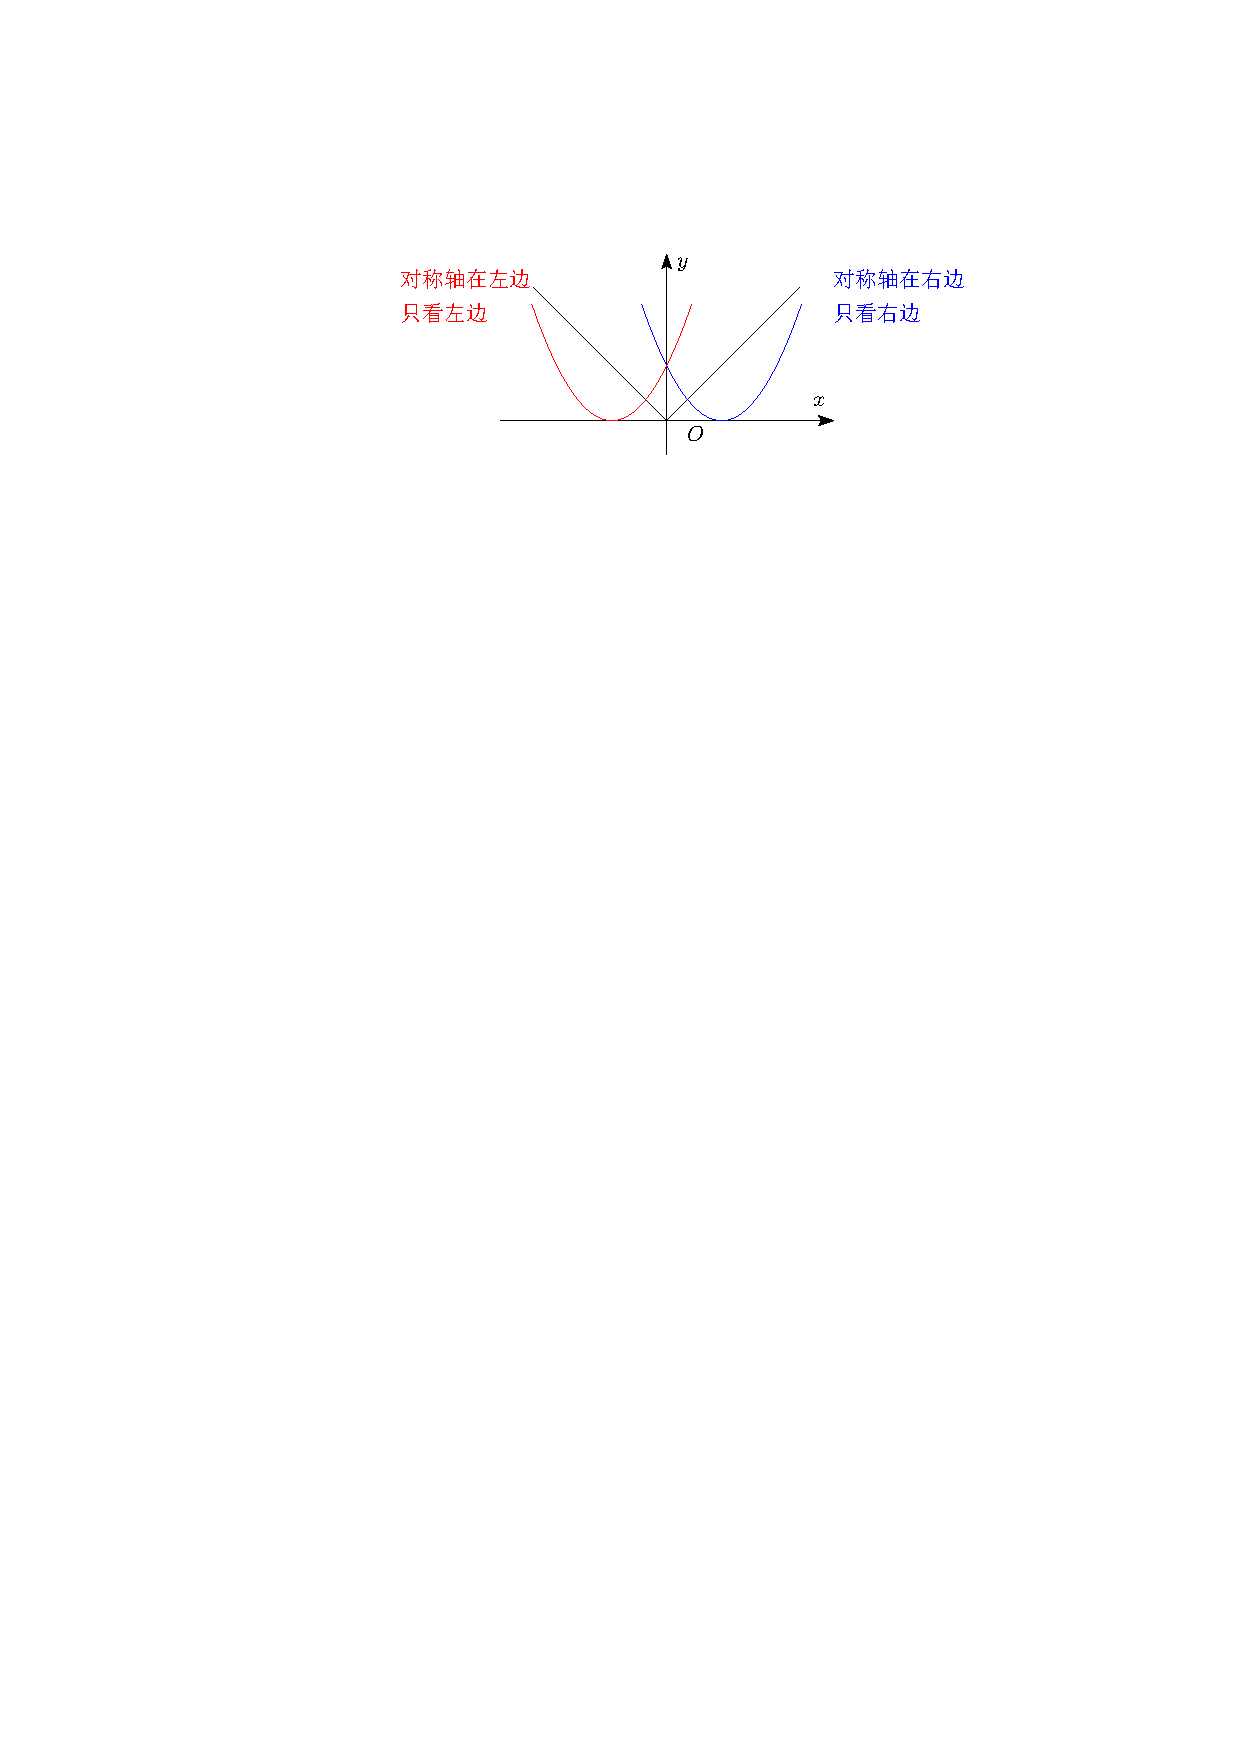
\includegraphics{image/可分离变量.pdf}
        \end{figure}
        最优解
        
        \[
            x_{i}^* = \left\{
                \begin{array}{ll}
                    0  & \text{若}|a_i|\leqslant \lambda\\
                    a_i-\operatorname{sgn(a_i)}\lambda & \text{若}|a_i|>\lambda
                \end{array}
            \right.
        \]
    \end{itemize}
    \item 图解法与实验法(手工作坊)
    \begin{itemize}
        \item 图解法:根据目标函数的图像求解 
        \item 实验法:依据一定规则对变量取不同的值,通过实验观察目标函数值的变化规律,找出问题的最优解。
    \end{itemize}
    \item 形式转化法:利用问题结构或最优性条件将其转化为有容易求解的另一类数学问题,然后对后者套用现有的方法求解。
    \item 数值迭代法:利用函数值或梯度信息按一定规则从一个点产生一个新的点,直到不能改进为止。得到的是数值解,是近似解。
    \begin{itemize}
        \item 模式搜索法:根据函数值变化规律探测函数的下降方向并沿着该方向寻求更优的点。
        \item 梯度方法:最优解、最优值未知。
    \end{itemize}
\end{enumerate}
\begin{note}
    线搜索方法:在每一步迭代,首先基于目标函数梯度信息产生搜索方向,然后沿该方向寻求目标函数的(近似)最小值点。重复上述过程,直到不能改进。
    \begin{enumerate}
        \item 取初始点$\boldsymbol{x}_0\in \mathbb{R}^n$,及有关参数. 令$k = 0$
        \item 验证停机准则.
        \item 计算当前迭代点$\boldsymbol{x}_k$的搜索方向$\boldsymbol{d}_k\in \mathbb{R}^n$
        \item 计算步长$\alpha_k>0$使满足
        \[
            f(\boldsymbol{x}_k+\alpha_k\boldsymbol{d}_k)<f(\boldsymbol{x}_k)
        \]    
        \[
            \alpha_k = \arg\min\limits_{\alpha_k>0}f(\boldsymbol{x}_k+\alpha_k+\boldsymbol{d}_k)
        \] 
        \item 令$\boldsymbol{x}_{k+1}=\boldsymbol{x}_k+\alpha_k\boldsymbol{d}_k$,转到第2步
    \end{enumerate}
\end{note}
\begin{note}
    信赖域方法:基于当前迭代点信息建立目标函数在该点邻域内的一个近似二次模型,然后将该模型小邻域内的最小值点作为新的迭代点。
    \[
        \begin{gathered}
            f(\boldsymbol{x}_{k}+\boldsymbol{d}) =f(x_{k})+\boldsymbol{d}^{\mathrm{T}}\nabla f(\boldsymbol{x}_{k})+\frac{1}{2}\boldsymbol{d}^{\mathrm{T}}\nabla^{2}f(\boldsymbol{x}_{k})\boldsymbol{d}+o(\|\boldsymbol{d}\|^{2}) \\
            \approx f(\boldsymbol{x}_{k})+\boldsymbol{d}^{\mathrm{T}}\nabla f(\boldsymbol{x}_{k})+\frac12\boldsymbol{d}^{\mathrm{T}}\nabla^{2}f(\boldsymbol{x}_{k})\boldsymbol{d} 
        \end{gathered}
    \]
    \[
        m_k(\boldsymbol{d})=f(\boldsymbol{x}_k)+\boldsymbol{d}^\mathrm{T}\nabla f(\boldsymbol{x}_k)+\frac{1}{2}\boldsymbol{d}^\mathrm{T}\boldsymbol{B}_k\boldsymbol{d}
    \]
    其中,$\boldsymbol{B}_k$为$\nabla^{2}f(\boldsymbol{x}_{k})$或近似
    \[
        \min_{\boldsymbol{d}\epsilon\mathbb{R}^n}f(\boldsymbol{x}_k+\boldsymbol{d})\Rightarrow\min\{m_k(\boldsymbol{d})\mid\boldsymbol{d}\in\mathbb{R}^n,\lVert\boldsymbol{d}\rVert\leqslant\Delta_k\}
    \]
    \[
        \boldsymbol{x}_{k+1} = \boldsymbol{x}_k+\boldsymbol{d}_k
    \]
\end{note}
\subsubsection{算法评价体系}
\begin{note}
    收敛性
    \begin{itemize}
        \item 全局收敛:从任意的初始点出发, 算法产生的迭代点列都收敛到问题的最优值点.
        \item 局部收敛:只有在初始点和最优值点具有某种程度的靠近时才能保证迭代点列收敛到最优值点.
        \item 弱收敛:迭代点列的某一聚点为优化问题的最优值点.
    \end{itemize}
\end{note}
\begin{note}
    收敛速度
    \begin{itemize}
        \item Q-收敛:前后两迭代点靠近最优值点的距离之比
        \[
            \lim\sup\limits_{k\to \infty}=\dfrac{\| \boldsymbol{x}_{k+1}-\boldsymbol{x}^{*} \|}{\|\boldsymbol{x}_{k}-\boldsymbol{x}^{*}\|}\leqslant q
        \]
        Q-线性收敛:$0<q<1$\newline
        Q-超线性收敛:$q = 0$\newline
        Q-r阶收敛:若存在$0\leqslant p<\infty$和$r\geqslant 1$
        \[
            \lim\sup\limits_{k\to \infty}=\dfrac{\| \boldsymbol{x}_{k+1}-\boldsymbol{x}^{*} \|}{\|\boldsymbol{x}_{k}-\boldsymbol{x}^{*}\|^r}\leqslant q
        \]
        $r$越大,收敛速度越快。若$r>1$,可推出其超线性收敛。
        \item R-线性收敛:借助一趋于零的等比数列度量迭代点收敛的快慢程度
        \[
            \| \boldsymbol{x}_{k}-\boldsymbol{x}^* \|\leqslant \kappa q^k,\ \kappa>0,q\in\left( 0,1 \right)
        \]
        R-超线性收敛:若存在$\kappa>0$和收敛于0的正数列$\left\{ q_k \right\}$
        \[
            \| \boldsymbol{x}_{k}-\boldsymbol{x}^* \|\leqslant \kappa\prod\limits_{i = 0}^{k}q_i
        \]
    \end{itemize}
    Q-(超)线性收敛$\Rightarrow$R-(超)线性收敛
\end{note}
\begin{example}
    证明无约束优化问题$\min\limits_{\boldsymbol{x}\in \mathbb{R}^n}f(\boldsymbol{x})$等价于下述约束优化问题
    \[
        \min\limits_{{\boldsymbol{x}\in \mathbb{R}^n},t\in \mathbb{R}}\left\{ t|t-f(\boldsymbol{x})\geqslant 0 \right\}
    \]
    \begin{proof}
        $\boldsymbol{x}^*$为无约束优化问题$\min\limits_{\boldsymbol{x}\in \mathbb{R}^n}f(\boldsymbol{x})$的最优解,当且仅当对任意的$\boldsymbol{x}\in\mathbb{R}^n,f(\boldsymbol{x})-f(\boldsymbol{x}^*)\geqslant 0$。所以优化问题
        \[
            \min\limits_{{\boldsymbol{x}\in \mathbb{R}^n},t\in \mathbb{R}}\left\{ t|t-f(\boldsymbol{x})\geqslant 0 \right\}
        \]
        的最优值为$f(\boldsymbol{x}^*)$。证毕!
    \end{proof}
\end{example}
\begin{example}
    设点列$\left\{ \boldsymbol{x}_k \right\}$Q-超线性收敛到$\boldsymbol{x}^*$,则
    \[
        \lim\limits_{k\to \infty}\dfrac{\| \boldsymbol{x}_{k+1}-\boldsymbol{x}_{k} \|}{\|\boldsymbol{x}_{k}-\boldsymbol{x}^{*}\|} = 1
    \]
    \begin{proof}
        设点列$\left\{ \boldsymbol{x}_k \right\}$Q-超线性收敛到$\boldsymbol{x}^*$,则
        \[
            \lim\limits_{k\to \infty}\dfrac{\| \boldsymbol{x}_{k+1}-\boldsymbol{x}^{*} \|}{\|\boldsymbol{x}_{k}-\boldsymbol{x}^{*}\|} = 0
        \]
        从而由三角不等式
        \[
            \begin{array}{ll}
                \lim\limits_{k\to \infty}\dfrac{\| \boldsymbol{x}_{k+1}-\boldsymbol{x}_{k} \|}{\| \boldsymbol{x}_{k}-\boldsymbol{x}^* \|}&\leqslant \dfrac{\| \boldsymbol{x}_{k+1}-\boldsymbol{x}^*\| + \| \boldsymbol{x}^*-\boldsymbol{x}_{k}  \|}{\| \boldsymbol{x}_{k}-\boldsymbol{x}^* \|}\\
                &=\lim\limits_{k\to \infty}\dfrac{\| \boldsymbol{x}_k-\boldsymbol{x}^* \|}{\| \boldsymbol{x}_k-\boldsymbol{x}^* \|} = 1
            \end{array}
        \]
        另一方面,
        \[
            \begin{array}{ll}
                \lim\limits_{k\to \infty}\dfrac{\| \boldsymbol{x}_{k+1}-\boldsymbol{x}_{k} \|}{\| \boldsymbol{x}_{k}-\boldsymbol{x}^* \|}&\geqslant \dfrac{\| \boldsymbol{x}^*-\boldsymbol{x}_{k}\| - \| \boldsymbol{x}_{k+1}-\boldsymbol{x}^*\|}{\| \boldsymbol{x}_{k}-\boldsymbol{x}^* \|}\\
                &=\lim\limits_{k\to \infty}\dfrac{\| \boldsymbol{x}_k-\boldsymbol{x}^* \|}{\| \boldsymbol{x}_k-\boldsymbol{x}^* \|} = 1
            \end{array}
        \]
        两式结合得命题结论。证毕!
    \end{proof}
\end{example}
\begin{example}
    用图解法求解下述优化问题的最优解
    \[
        \min\left\{ x_1+x_2|x_1^2+x_2^2\leqslant 2 \right\}
    \]
    \begin{figure}[htbp]
        \centering
        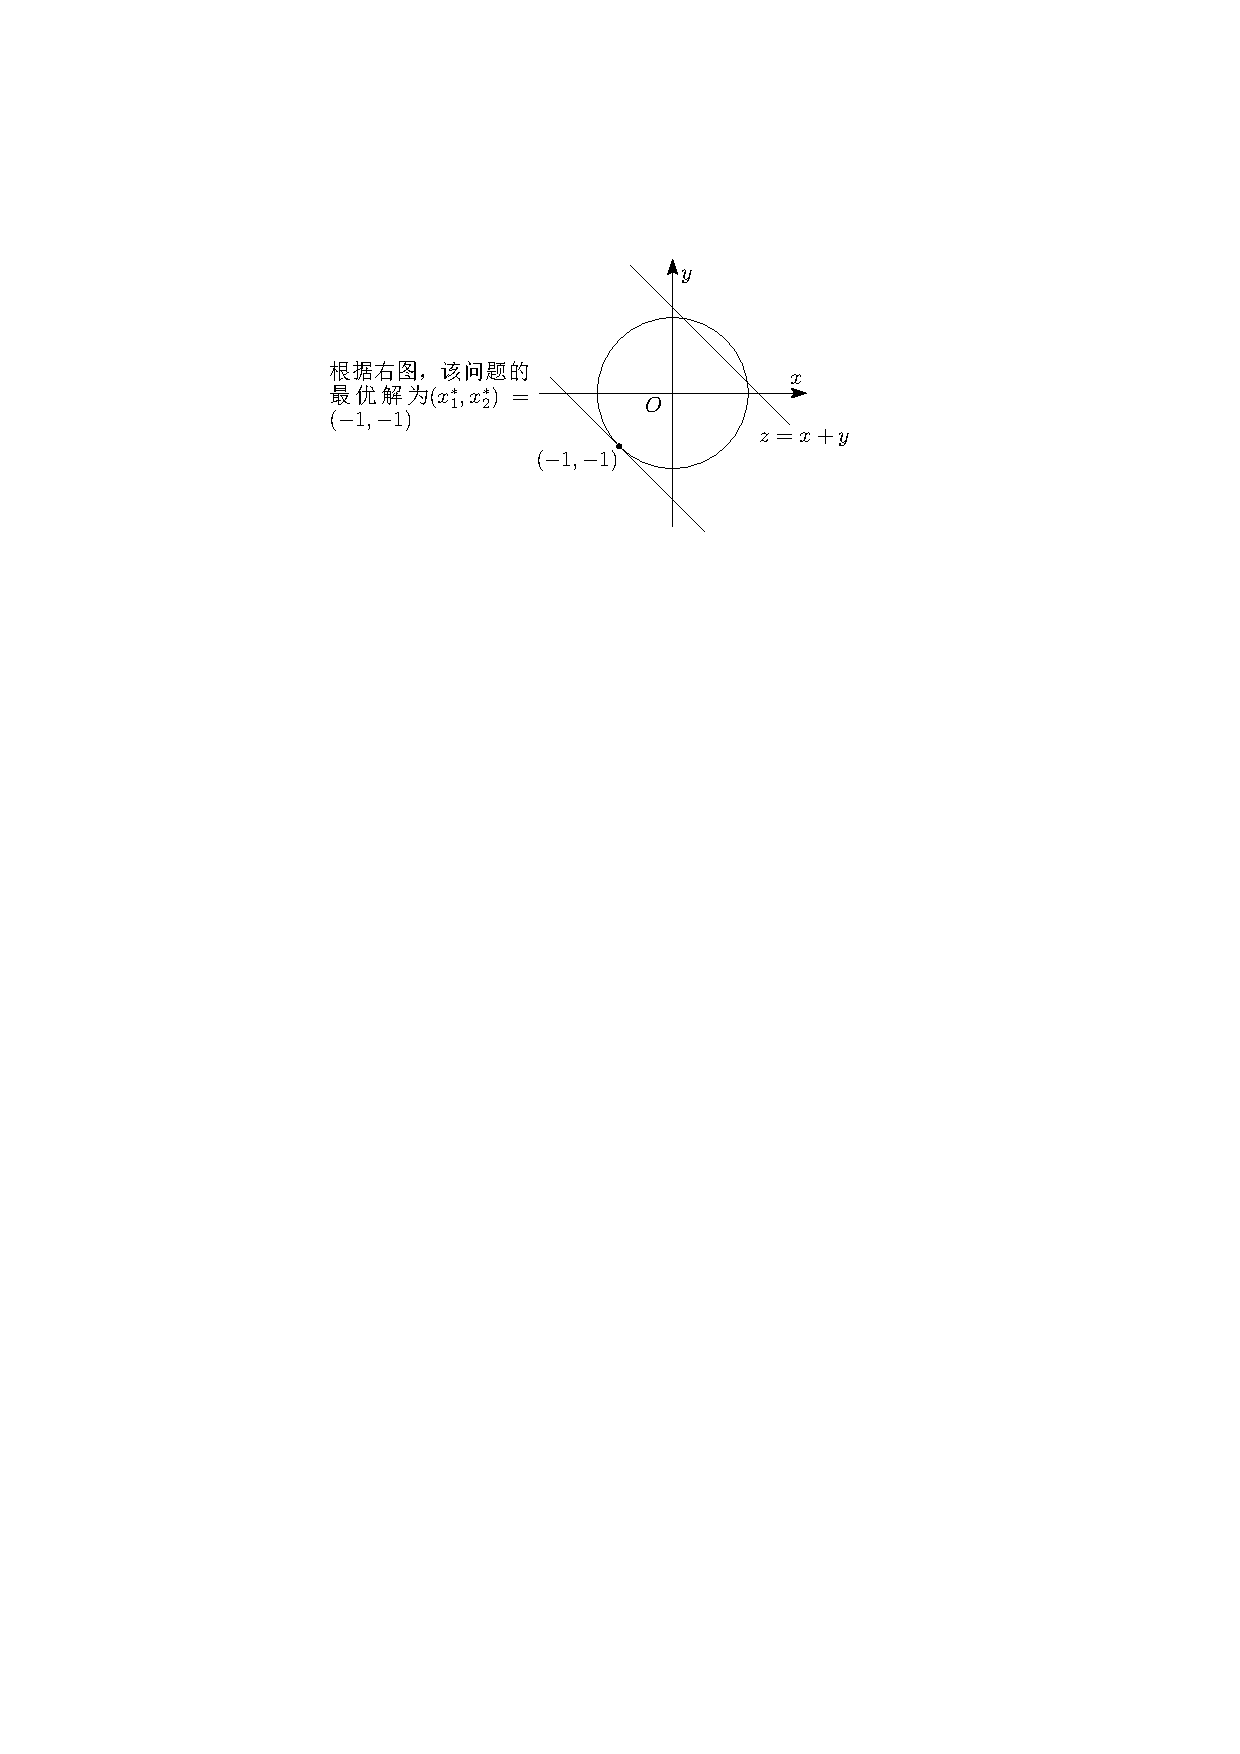
\includegraphics{image/习题-图解法最优.pdf}
    \end{figure}
\end{example}
\begin{example}
    设$\boldsymbol{a}\in\mathbb{R}^n,\kappa>0\|\boldsymbol{a}\|>1$,试求解优化问题
    \[
        \begin{array}{rl}
            \min & \|x\|\\
            \operatorname{s.t.} & \|\boldsymbol{x}\|-\boldsymbol{a}^{\mathrm{T}}\boldsymbol{x}+\kappa\leqslant 0
        \end{array}
    \]
    解:
    由Cauchy-Scwarzy不等式,对同样长度的$\boldsymbol{x}$,$\boldsymbol{x}$与$\boldsymbol{a}$同向时达到最小,$\boldsymbol{x}$的取值范围达到最大。故该优化问题的最优解满足$\boldsymbol{x} = t\boldsymbol{a}$,其中$t>0$待定。故上述优化问题化为
    \[
        \begin{array}{rl}
            \min & t\|a\|\\
            \operatorname{s.t.} & t\|\boldsymbol{a}\|-t\|\boldsymbol{a}\|^2+\kappa\leqslant 0
        \end{array}
    \]
    即
    \[
        \begin{array}{rl}
            \min & t\|a\|\\
            \operatorname{s.t.} & t\geqslant\dfrac{\kappa}{\|\boldsymbol{a}\|^2-\|\boldsymbol{a}\|}
        \end{array}
    \]
    显然,其最优解为$t^* = \dfrac{\kappa}{\|\boldsymbol{a}\|^2-\|\boldsymbol{a}\|}$。这样,原问题的最优解为
    \[
        \boldsymbol{x}^* = t^*\boldsymbol{a} = \dfrac{\kappa a}{\|\boldsymbol{a}\|^2-\|\boldsymbol{a}\|}
    \]
\end{example}
\begin{example}
    设$\boldsymbol{a}\in\mathbb{R}^n,\rho>0$,矩阵$\boldsymbol{\Sigma}_0\succ0$(对称正定)。试用解析法求解如下优化问题。
    \[
        \begin{array}{rl}
            \max\limits_{\boldsymbol{\Sigma}\succ 0} & \boldsymbol{a}^{\mathrm{T}}\boldsymbol{\Sigma}\boldsymbol{a}\\
            \operatorname{s.t.} & \|\boldsymbol{\Sigma}-\boldsymbol{\Sigma}\|_{\mathrm{F}}\leqslant \rho
        \end{array}
    \]

    解:令$\Delta\boldsymbol{\Sigma} = \boldsymbol{\Sigma}-\boldsymbol{\Sigma}_0$,则
    原优化问题转化为
    \[
        \begin{array}{rl}
            \max & \boldsymbol{a}^{\mathrm{T}}\Delta\boldsymbol{\Sigma}\boldsymbol{a}+\boldsymbol{a}^{\mathrm{T}}\boldsymbol{\Sigma}_0\boldsymbol{a}\\
            \operatorname{s.t.} & \|\Delta\boldsymbol{\Sigma}\|_{\mathrm{F}}\leqslant \rho
        \end{array}
    \]
    由Cauchy-Scwarzy不等式:
    \[
        \boldsymbol{a}^{\mathrm{T}}\Delta\boldsymbol{\Sigma}\boldsymbol{a} = \left< \Delta\boldsymbol{\Sigma},\boldsymbol{a}\boldsymbol{a}^{\mathrm{T}} \right>\leqslant \|\Delta\boldsymbol{\Sigma}\|_{\mathrm{F}}\|\boldsymbol{a}\boldsymbol{a}^{\mathrm{T}}\|_{\mathrm{F}}\leqslant \rho\|\boldsymbol{a}\boldsymbol{a}^{\mathrm{T}}\|_{\mathrm{F}}
    \]
    当且仅当$\Delta\boldsymbol{\Sigma}$与$\boldsymbol{a}\boldsymbol{a}^{\mathrm{T}}$方向一致时取等号,当$\|\Delta\boldsymbol{\Sigma}\|_{\mathrm{F}} = \rho$是取最优值。

    原问题的最优解为
    \[
        \boldsymbol{\Sigma}^{*} = \boldsymbol{\Sigma}_0+\rho\dfrac{\boldsymbol{a}\boldsymbol{a}^{\mathrm{T}}}{\|\boldsymbol{a}\boldsymbol{a}^{\mathrm{T}}\|}
    \]
    上述问题的最优解为
    \[
        \boldsymbol{a}^{\mathrm{T}}\boldsymbol{\Sigma}^*\boldsymbol{a} = \boldsymbol{a}^{\mathrm{T}}\boldsymbol{\Sigma}_0\boldsymbol{a} + \rho\boldsymbol{a}^{\mathrm{T}}\boldsymbol{a}
    \]
\end{example}

